\documentclass[conference]{IEEEtran}
\IEEEoverridecommandlockouts
\usepackage{cite}
\usepackage{amsmath,amssymb}
\usepackage{graphicx}
\usepackage{booktabs}
\usepackage{multirow}
\usepackage{url}
\usepackage{array}
\usepackage{tikz}
\usetikzlibrary{arrows.meta,positioning}
\usepackage{xcolor}
\usepackage{float}

\begin{document}

\title{Automatic Detection and Classification System of Domestic Waste via a Cascaded YOLOv8 and ResNet-101 Convolutional Neural Network}

\author{\IEEEauthorblockN{Mrityunjay Yadav}
\IEEEauthorblockA{Department of Information Technology\\
Netaji Subhas University of Technology (NSUT)\\
New Delhi, India\\
Email: mrityunjay@example.com}
\and
\IEEEauthorblockN{Gaurav Yadav}
\IEEEauthorblockA{Department of Information Technology\\
Netaji Subhas University of Technology (NSUT)\\
New Delhi, India\\
Email: gaurav@example.com}}

\maketitle

\begin{abstract}
Automated waste detection and classification can support efficient waste segregation and recycling. This paper investigates a two-stage computer-vision pipeline that combines YOLOv8 object detection with ResNet-101 crop classification, evaluated on the Trash-Detection-14 dataset. The detector first predicts candidate bounding boxes and waste categories. Each detected region is then cropped and passed to ResNet-101. In the evaluated cascaded configuration, a detection is retained only when the ResNet-101 prediction agrees with the original YOLOv8 class. The system recognizes five categories: glass, metal, paper, plastic, and waste. Both approaches were evaluated on the same set of 110 test images. Standalone YOLOv8 achieved a precision of 0.6571, recall of 0.5257, mAP@0.5 of 0.4678, and mAP@0.5:0.95 of 0.4338. The agreement-based cascade increased precision to 0.8980 and reduced false positives from 48 to 10, while recall decreased slightly to 0.5029. The cascade also increased average inference time from 0.0107 to 0.0304 seconds per image. These results indicate a precision--recall and latency trade-off: agreement filtering removes many false detections but also rejects some correct detections.
\end{abstract}

\begin{IEEEkeywords}
waste detection, cascaded CNN, YOLOv8, ResNet-101, object detection, image classification, waste segregation, deep learning
\end{IEEEkeywords}

\section{Introduction}
Waste generation has increased with urbanization, population growth, and changing consumption patterns. Effective segregation is important for recycling, resource recovery, and reducing the amount of waste sent to landfills. Manual sorting can be time-consuming and may be inconsistent, particularly when waste items overlap or appear against cluttered backgrounds.

Computer vision and deep learning provide methods for automating visual recognition. Image classification assigns a category to an image or image region, while object detection additionally predicts object locations. YOLO-family detectors perform localization and classification in a unified model and are widely used in real-time detection tasks \cite{redmon2016yolo,jocher2023yolov8}.

This work investigates a two-stage approach for domestic waste recognition. YOLOv8 first detects candidate objects. The detected regions are then cropped and classified independently using ResNet-101. The evaluated second-stage rule retains a detection only when the class predicted by ResNet-101 agrees with the YOLOv8 class. Thus, the second stage acts as a verification filter; it does not replace the YOLOv8 label with a different ResNet-101 label.

The main contributions are:
\begin{itemize}
  \item implementation of a YOLOv8-based detector for five waste categories;
  \item integration of ResNet-101 as a crop-level classification verifier;
  \item comparison of standalone detection and agreement-based cascaded inference on the same 110 test images; and
  \item analysis of precision, recall, average precision, false positives, false negatives, and inference time.
\end{itemize}

\section{Related Work}
Deep learning methods have been applied to waste classification and detection. Early work on recyclable-waste classification used the TrashNet image set to assign a single label to each image \cite{yang2016trashnet}. Object detectors such as Faster R-CNN \cite{ren2017fasterrcnn} and YOLO \cite{redmon2016yolo} additionally estimate object locations, enabling multiple items in a single image to be identified.

Residual Networks (ResNets), introduced by He \textit{et al.}, use shortcut connections to support the training of deep neural networks \cite{he2016resnet}. ResNet-101 is a deep convolutional architecture suitable for extracting image features for classification, and pretrained ImageNet weights \cite{deng2009imagenet} are commonly used to initialize it.

YOLO is a family of unified object detection models. The Ultralytics implementation provides YOLOv8 detection models and associated training and inference tools \cite{jocher2023yolov8,ultralytics}. Detection followed by a separate classification stage is a common cascade design. The present study explores a two-model cascade using YOLOv8 and ResNet-101 for domestic waste.

\section{Dataset Description}
The object-detection dataset used in this study is the Trash-Detection-14 dataset obtained from Roboflow Universe \cite{roboflow}. The annotations are provided in a YOLO-compatible format. The test split used here contains 110 images with 175 annotated objects (true positives plus false negatives in Table~\ref{tab:overall}).

Five classes are used, as listed in Table~\ref{tab:classes}.
\begin{table}[htbp]
\caption{Waste Categories}
\label{tab:classes}
\centering
\begin{tabular}{cc}
\toprule
\textbf{Class ID} & \textbf{Category}\\
\midrule
0 & Glass\\
1 & Metal\\
2 & Paper\\
3 & Plastic\\
4 & Waste\\
\bottomrule
\end{tabular}
\end{table}

For ResNet-101 training, object image patches were organized into the corresponding class directories. The recorded classifier split contains 13,042 training patches, 1,414 validation patches, and 175 test patches. The patches were cropped from annotated objects of the Trash-Detection-14 dataset. No other detector or classifier architecture is used in this work.

\section{Proposed Methodology}
Two approaches are evaluated.

\subsection{Approach 1: Standalone YOLOv8 Detection}
In the baseline approach, an input image is passed directly to the trained YOLOv8 detector. The model predicts bounding boxes, class labels, and confidence scores for detected objects. The detector is trained to recognize the five waste categories.

\subsection{Approach 2: YOLOv8 with ResNet-101 Verification}
\label{sec:approach2}
The cascaded approach consists of the following stages:
\begin{enumerate}
  \item \textbf{Detection:} YOLOv8 predicts candidate bounding boxes and preliminary class labels.
  \item \textbf{Cropping:} Each predicted bounding box is used to extract a region from the original image, with coordinates constrained to image boundaries.
  \item \textbf{Preprocessing:} Each crop is resized to $224\times224$ pixels and normalized using ImageNet channel statistics (mean $[0.485,0.456,0.406]$ and standard deviation $[0.229,0.224,0.225]$), as used by the inference preprocessing pipeline.
  \item \textbf{Classification:} ResNet-101 predicts one of the five waste categories for each crop.
  \item \textbf{Verification:} The ResNet-101 prediction is compared with the YOLOv8 label. A detection is retained only when the two predicted classes agree.
\end{enumerate}

The cascade uses bounding boxes generated by YOLOv8; ResNet-101 performs crop classification and does not independently generate object locations. Consequently, objects missed by YOLOv8 cannot be recovered by the second stage. The agreement rule can reject false positives, but it can also reject true positives when either model predicts an incorrect class.

\subsection{Pipeline Overview}
The inference sequence is shown in Fig.~\ref{fig:pipeline}.
\begin{figure}[htbp]
\centering
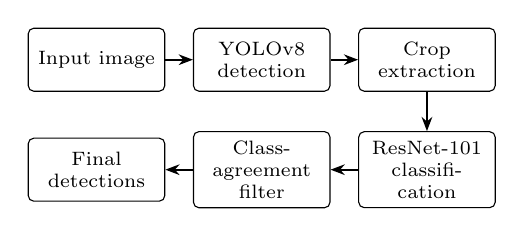
\begin{tikzpicture}[
  node distance=3.5mm,
  box/.style={draw, rounded corners=2pt, align=center, font=\scriptsize, minimum height=8mm, text width=15mm},
  arr/.style={-{Stealth[length=1.8mm]}, thick}]
\node[box] (a) {Input image};
\node[box, right=of a] (b) {YOLOv8 detection};
\node[box, right=of b] (c) {Crop extraction};
\node[box, below=5mm of c] (d) {ResNet-101 classification};
\node[box, left=of d] (e) {Class-agreement filter};
\node[box, left=of e] (f) {Final detections};
\draw[arr] (a)--(b); \draw[arr] (b)--(c); \draw[arr] (c)--(d);
\draw[arr] (d)--(e); \draw[arr] (e)--(f);
\end{tikzpicture}
\caption{Inference pipeline of the YOLOv8 + ResNet-101 cascade.}
\label{fig:pipeline}
\end{figure}

\section{Model Implementation}
\subsection{YOLOv8 Detector}
The YOLOv8 model was trained using the annotated waste-detection dataset, and the selected checkpoint was saved as \texttt{best.pt}. The detector is responsible for object localization and initial category prediction. The training hyperparameters of the detector are summarized in Table~\ref{tab:implementation}.

\subsection{ResNet-101 Classifier}
ResNet-101 was adapted for five-class classification by replacing its final classification layer. The trained classifier checkpoint was saved as \texttt{best\_resnet101.pth}. The classifier receives resized object crops. The inference preprocessing uses a $224\times224$ input and ImageNet normalization. The best validation macro F1-score reached during training was 0.5971.

\subsection{Implementation Environment}
The project was developed using Python, PyTorch \cite{paszke2019pytorch}, Torchvision, and Ultralytics. The software environment comprised Python 3.13.15, PyTorch 2.11.0+cu130, and Ultralytics 8.4.175, and experiments ran on an NVIDIA Tesla T4 GPU.

\begin{table}[htbp]
\caption{Implementation Details}
\label{tab:implementation}
\centering
\small
\begin{tabular}{>{\raggedright\arraybackslash}p{0.38\columnwidth}>{\raggedright\arraybackslash}p{0.52\columnwidth}}
\toprule
\textbf{Parameter} & \textbf{Value}\\
\midrule
YOLOv8 variant & \textbf{[to be filled]}\\
YOLOv8 input size & \textbf{[to be filled]}\\
YOLOv8 epochs & \textbf{[to be filled]}\\
Batch size, optimizer & \textbf{[to be filled]}\\
Learning rate, scheduler & \textbf{[to be filled]}\\
ResNet-101 input size & $224\times224$ pixels\\
ResNet-101 normalization & ImageNet mean/std\\
GPU & NVIDIA Tesla T4\\
Python & 3.13.15\\
PyTorch & 2.11.0+cu130\\
Ultralytics & 8.4.175\\
\bottomrule
\end{tabular}
\end{table}

\section{Experimental Results}
\subsection{Evaluation Setup}
Both approaches were evaluated on the same 110 test images using the same class mapping and ground-truth annotations. The evaluation output reports precision, recall, mAP@0.5, mAP@0.5:0.95, true positives (TP), false positives (FP), false negatives (FN), and average inference time per image. The cascaded approach applies the class-agreement filter described in Section~\ref{sec:approach2}.

\subsection{Overall Detection Comparison}
Table~\ref{tab:overall} reports the measured results of the evaluation run.
\begin{table}[H]
\caption{Overall Metric Comparison on 110 Test Images (time in seconds per image)}
\label{tab:overall}
\centering
\footnotesize
\setlength{\tabcolsep}{2.5pt}
\resizebox{\columnwidth}{!}{%
\begin{tabular}{lccccccccc}
\toprule
\textbf{Approach} & \textbf{Precision} & \textbf{Recall} & \textbf{mAP@0.5} & \textbf{mAP@0.5:0.95} & \textbf{Time (s)} & \textbf{TP} & \textbf{FP} & \textbf{FN}\\
\midrule
YOLOv8 & 0.6571 & 0.5257 & 0.4678 & 0.4338 & 0.0107 & 92 & 48 & 83\\
YOLOv8 + ResNet-101 & 0.8980 & 0.5029 & 0.4533 & 0.4193 & 0.0304 & 88 & 10 & 87\\
\bottomrule
\end{tabular}}
\end{table}

The verification stage increased precision from 0.6571 to 0.8980, an absolute increase of 0.2409. The number of false positives decreased from 48 to 10. However, recall decreased from 0.5257 to 0.5029, while false negatives increased from 83 to 87. The mAP@0.5 decreased from 0.4678 to 0.4533, and mAP@0.5:0.95 decreased from 0.4338 to 0.4193. Average inference time increased from 0.0107 to 0.0304 seconds per image. Thus, the measured result supports a precision improvement and false-positive reduction, but not an overall improvement across all detection metrics.

\subsection{Per-Class AP@0.5}
Per-class AP@0.5 values from the same evaluation are given in Table~\ref{tab:classap}.
\begin{table}[H]
\caption{Per-Class AP@0.5 Comparison}
\label{tab:classap}
\centering
\begin{tabular}{lcc}
\toprule
\textbf{Class} & \textbf{YOLOv8} & \textbf{YOLOv8 + ResNet-101}\\
\midrule
Glass & 0.4651 & 0.4500\\
Metal & 0.6270 & 0.6376\\
Paper & 0.6019 & 0.5556\\
Plastic & 0.6452 & 0.6235\\
Waste & 0.0000 & 0.0000\\
\bottomrule
\end{tabular}
\end{table}

The verification stage improved AP@0.5 slightly for the Metal category, while AP@0.5 decreased for Glass, Paper, and Plastic. Both approaches recorded zero AP@0.5 for Waste in this evaluation. This indicates that the Waste category requires further investigation, including review of class-specific annotations, predictions, class mapping, and the number of test instances.

\section{Discussion}
The evaluation demonstrates that strict class-agreement filtering can make predictions more conservative. In this experiment, it substantially reduced false positives and increased precision. At the same time, it rejected some detections that would otherwise have been counted as true positives, resulting in lower recall and slightly lower mAP values. The extra ResNet-101 pass also increased average inference time by approximately 2.84 times (0.0304/0.0107).

These results should not be interpreted as evidence that ResNet-101 corrects YOLOv8 labels: the evaluated rule retains detections only when both models agree, and it does not substitute the ResNet-101 class when the predictions differ. The second stage cannot recover objects missed by YOLOv8 because it processes only YOLOv8 proposals. Performance may also be affected by crop quality, class imbalance, differences between classifier training patches and detector-generated crops, and the quality of ground-truth annotations.

The zero AP@0.5 for the Waste category in both approaches deserves specific review. A class-wise confusion matrix and counts of ground-truth instances and predictions would help determine whether this result is caused by limited representation, annotation issues, or model failure. The reported inference times depend on the hardware, batch size, image loading, and timing procedure.

\section{Conclusion and Future Work}
This paper presented a waste detection and classification pipeline based on YOLOv8 and ResNet-101. The first approach uses YOLOv8 as a standalone detector, while the second adds a ResNet-101 classifier to verify the categories of detected object crops through strict class-agreement filtering. On 110 test images, standalone YOLOv8 achieved precision 0.6571, recall 0.5257, mAP@0.5 0.4678, and mAP@0.5:0.95 0.4338. The cascaded approach achieved precision 0.8980 and reduced false positives from 48 to 10, but recall and both mAP measures decreased, and average inference time increased.

The findings show that the proposed verification stage is useful when reducing false positives is more important than retaining every possible detection. Future work includes improving class balance, investigating the Waste category, refining crop extraction and preprocessing, exploring confidence-aware verification rather than strict label agreement, and evaluating the approach on a larger independent test set.

\section*{Acknowledgment}
The authors thank the Department of Information Technology, Netaji Subhas University of Technology (NSUT), for its guidance and support.

\begin{thebibliography}{00}
\bibitem{he2016resnet}
K. He, X. Zhang, S. Ren, and J. Sun, ``Deep residual learning for image recognition,'' in \emph{Proc. IEEE Conf. Computer Vision and Pattern Recognition (CVPR)}, 2016, pp. 770--778.

\bibitem{redmon2016yolo}
J. Redmon, S. Divvala, R. Girshick, and A. Farhadi, ``You only look once: Unified, real-time object detection,'' in \emph{Proc. IEEE Conf. Computer Vision and Pattern Recognition (CVPR)}, 2016, pp. 779--788.

\bibitem{ren2017fasterrcnn}
S. Ren, K. He, R. Girshick, and J. Sun, ``Faster R-CNN: Towards real-time object detection with region proposal networks,'' \emph{IEEE Trans. Pattern Anal. Mach. Intell.}, vol. 39, no. 6, pp. 1137--1149, Jun. 2017.

\bibitem{jocher2023yolov8}
G. Jocher, A. Chaurasia, and J. Qiu, ``Ultralytics YOLOv8,'' 2023. [Online]. Available: \url{https://github.com/ultralytics/ultralytics}

\bibitem{ultralytics}
Ultralytics, ``Ultralytics YOLO documentation.'' [Online]. Available: \url{https://docs.ultralytics.com/}. Accessed: Nov. 20, 2026.

\bibitem{yang2016trashnet}
M. Yang and G. Thung, ``Classification of trash for recyclability status,'' Stanford Univ., CS229 Project Report, 2016.

\bibitem{deng2009imagenet}
J. Deng, W. Dong, R. Socher, L.-J. Li, K. Li, and L. Fei-Fei, ``ImageNet: A large-scale hierarchical image database,'' in \emph{Proc. IEEE Conf. Computer Vision and Pattern Recognition (CVPR)}, 2009, pp. 248--255.

\bibitem{paszke2019pytorch}
A. Paszke \emph{et al.}, ``PyTorch: An imperative style, high-performance deep learning library,'' in \emph{Advances in Neural Information Processing Systems (NeurIPS)}, vol. 32, 2019.

\bibitem{roboflow}
Roboflow Universe, ``Trash-Detection-14 dataset.'' [Online]. Available: \url{https://universe.roboflow.com/}
\end{thebibliography}

\end{document}
